\section{STM32}

\begin{frame}{Introduksjon}
	
	\begin{figure}
		\centering
		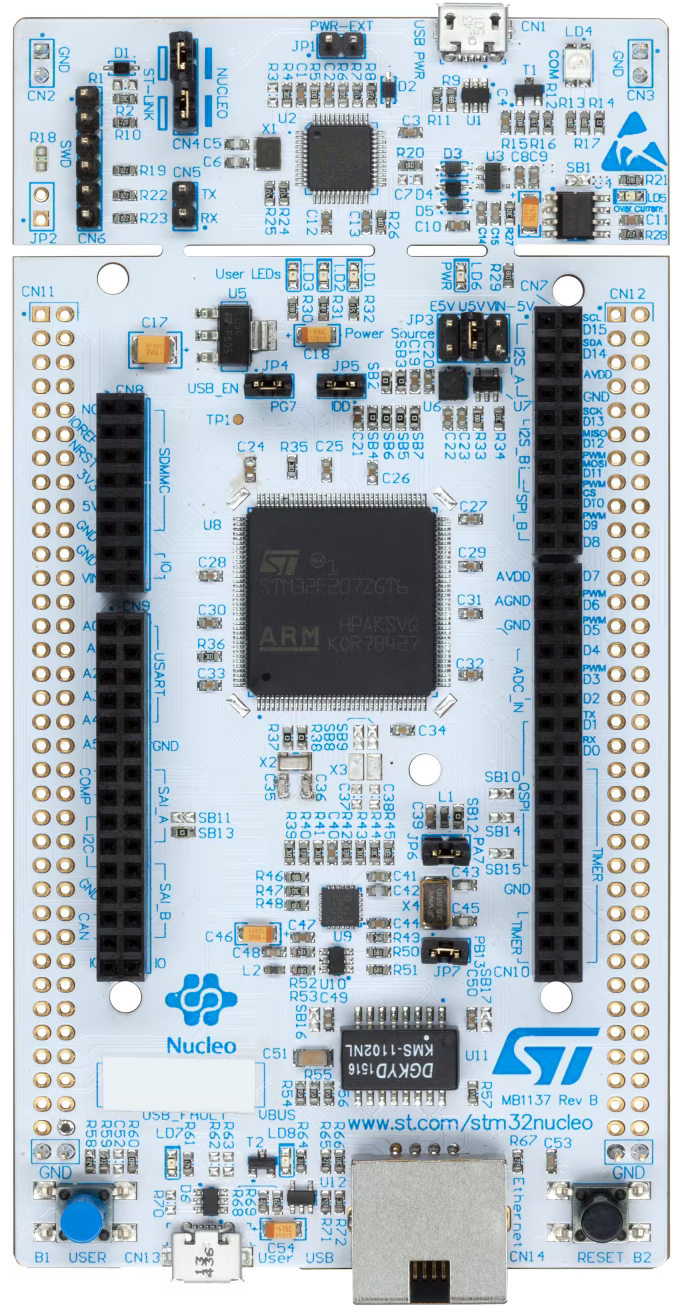
\includegraphics[width=0.5\linewidth,angle=90]{img/nucleo-f767zi}
		\caption{Nucleo-F767ZI}
		\label{fig:nucleo-f767zi}
	\end{figure}
	
	
\end{frame}


\begin{frame}{Introduksjon}

Mikrokontrolleren har mange innebygde funksjonar i hardware:

\begin{itemize}
	\item Flyttalsstøtte (FPU)
	\item 12-bit Analog til digital omformar (ADC)
	\item 12-bit Digital til analog omformar (DAC)
\end{itemize}

	
\end{frame}

\begin{frame}[containsverbatim]{Klokketreet}
	
\begin{figure}
	\centering
	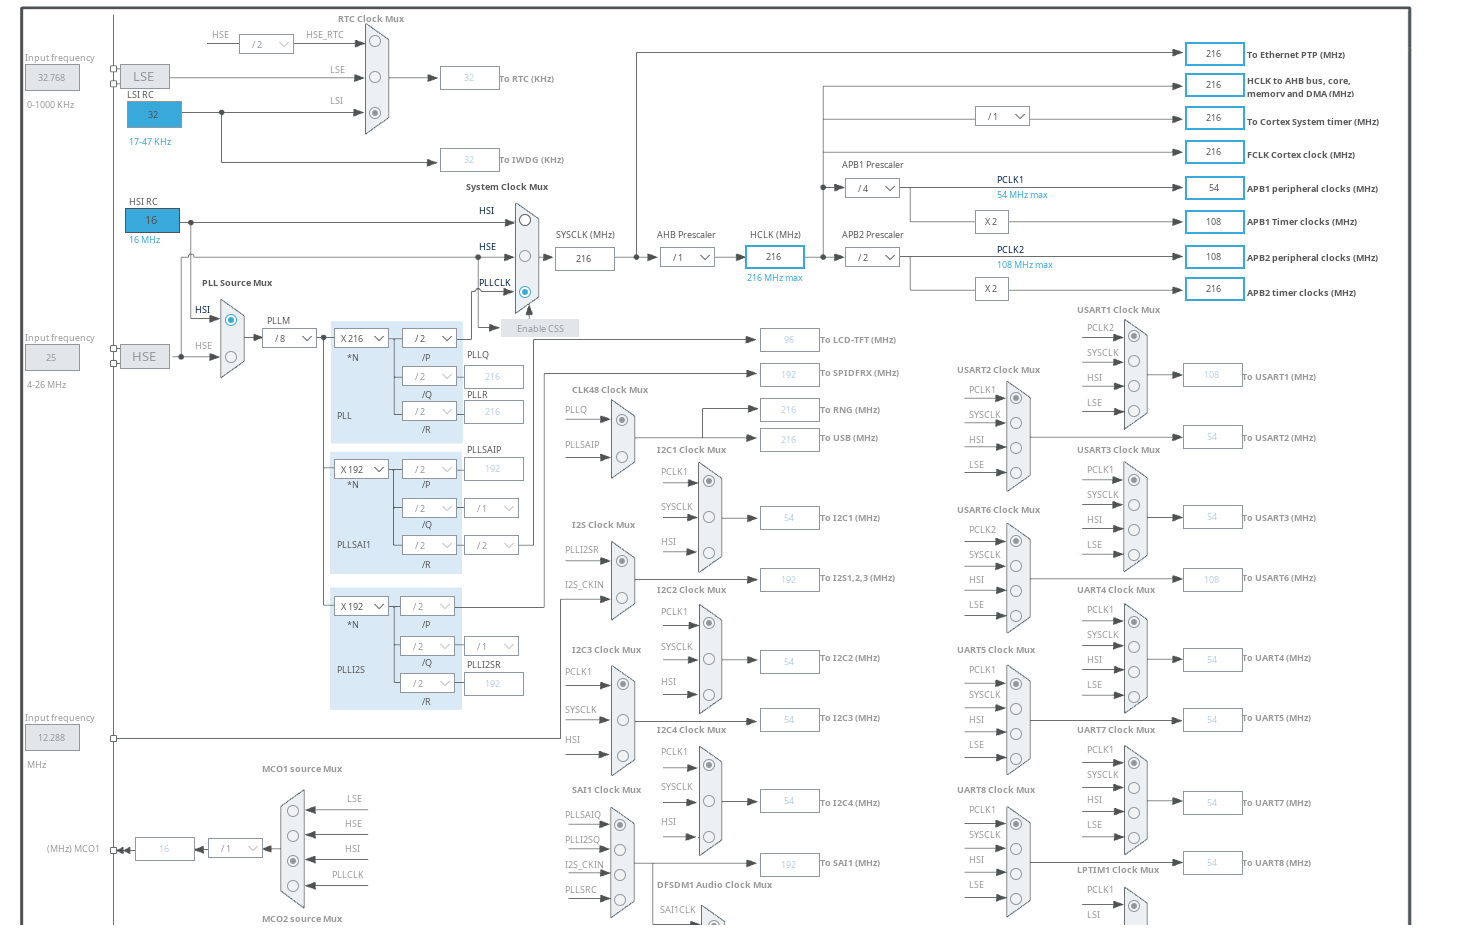
\includegraphics[width=0.95\linewidth]{img/clock-tree}
	\caption{Utdrag frå klokketreet til STM32F767}
	\label{fig:clock-tree}
\end{figure}

	
\end{frame}

\begin{frame}{Kretsskjema}
	
\begin{figure}
	\centering
	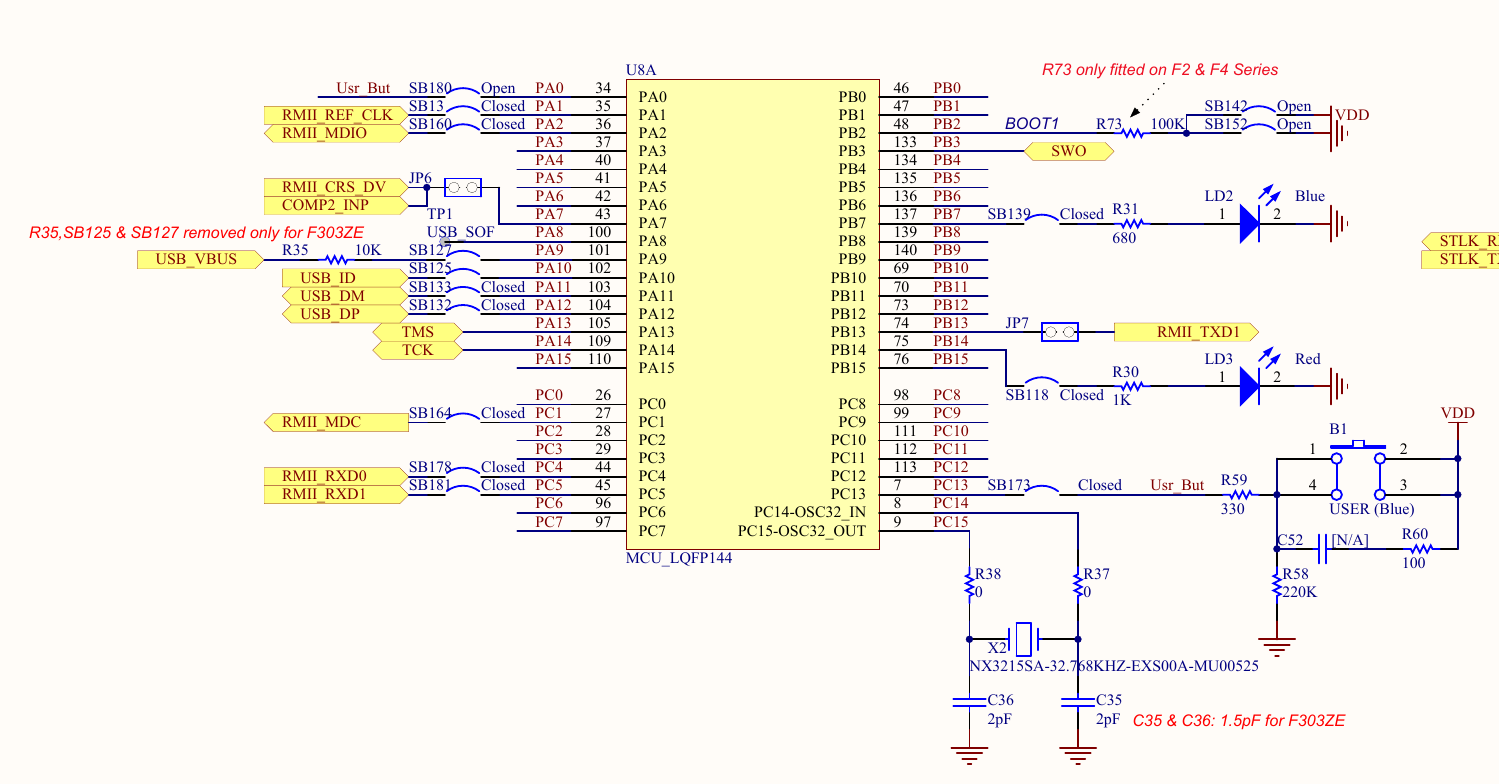
\includegraphics[width=0.95\linewidth]{img/schematic-user-led-and-pb}
	\caption{Tilkopling for trykknapp og lysdiodar}
	\label{fig:schematic-user-led-and-pb}
\end{figure}

	
	
\end{frame}


\begin{frame}{Kretsskjema}
	
\begin{figure}
	\centering
	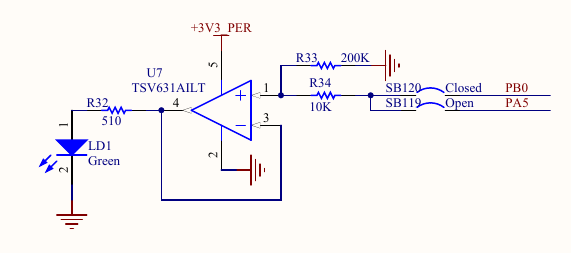
\includegraphics[width=0.7\linewidth]{img/schematic-user-led1-amplifier}
	\caption{Lysdioden LD1 er av ein eller anna grunn kopla til ein forsterkar}
	\label{fig:schematic-user-led1-amplifier}
\end{figure}

	
	
\end{frame}







\begin{frame}{Kretsskjema}
	
\begin{columns}[c]
	% create the column with the first image, that occupies
	% half of the slide
	\begin{column}{.5\textwidth}
		\begin{figure}
			\centering
				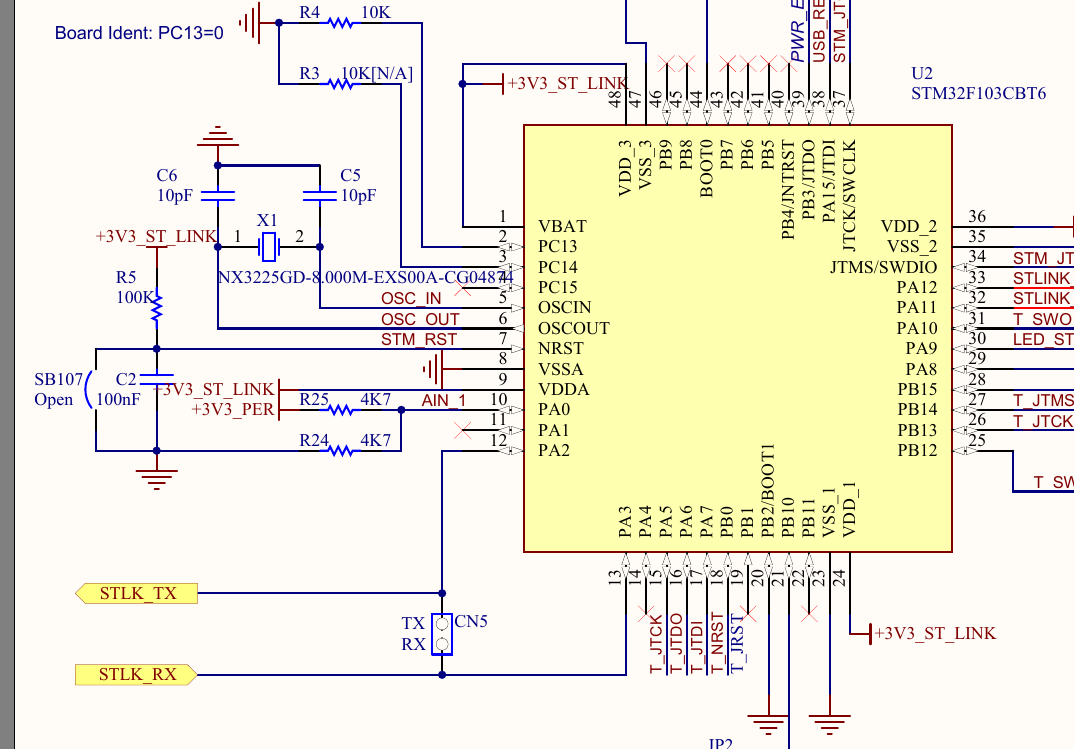
\includegraphics[width=0.95\linewidth]{img/stlink-uart}
			\caption{Tilkopling for UART på STLink}
		\end{figure}      
	\end{column}
	% create the column with the second image, that also
	% occupies half of the slide
	\begin{column}{.5\textwidth}
		\begin{figure}
			\centering
				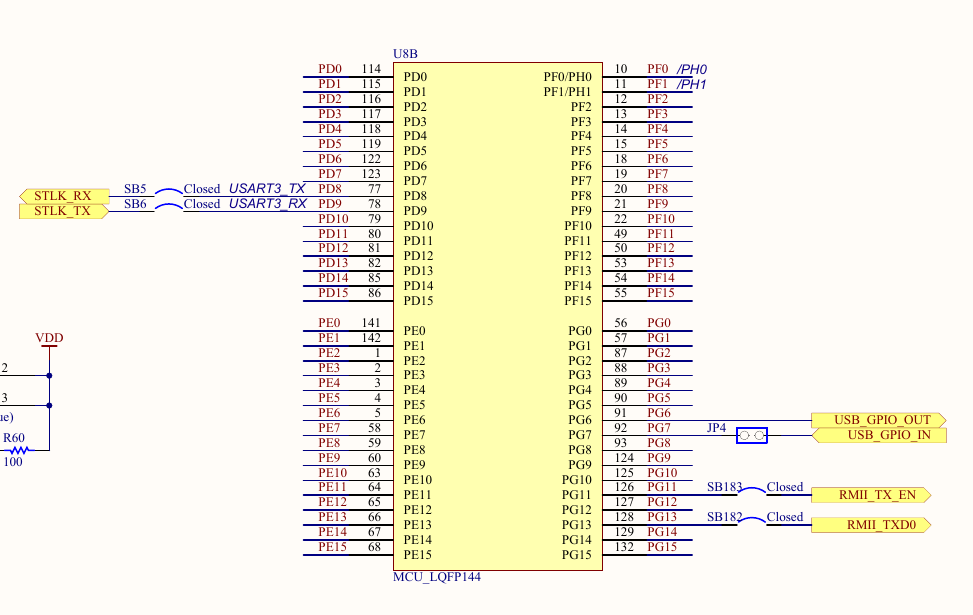
\includegraphics[width=0.95\linewidth]{img/mcu-uart}
			\caption{Tilkopling for UART på mikrokontrolleren}
		\end{figure}
	\end{column}
\end{columns}
	
\end{frame}


\begin{frame}[containsverbatim]{VSCode og PlatformIO}
	
...
	
	
\end{frame}